\scanpage{48}
% loc: item 4, heading and opening
\textcircled{4} \inserted{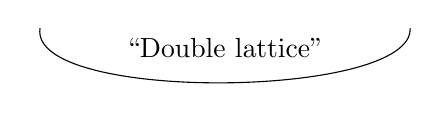
\begin{tikzpicture}[baseline=(n.base)]\node (n) {``\uline{Double lattice}''};\draw (-2.35,0.25) .. controls (-2.5,-0.7) and (2.4,-0.65) .. (2.35,0.25);\end{tikzpicture}} Suppose $S=\operatorname{Spec}k$, $k\subset\mathbb C$ \uline{algebraic} extension of $\mathbb Q$. Consider the functor which to $M$ associated
% loc: first labeled display
\begingroup\makeatletter\tagsleft@true\makeatother
\[
\bigl\{T_{\mathrm{DR}}(M),T_{\mathrm B}(M),\varphi_M\bigr\} \tag*{(4.1)}
\]
\endgroup
% loc: first comparison and question
where $\varphi:T_{\mathrm B}(M)\unsure{\otimes|\ominus}_{\mathbb Q}\mathbb C\simeq T_{\mathrm{DR}}(M)\unsure{\otimes|\ominus}_k\mathbb C$ ; here, one does not consider $T_{\mathrm{DR}}(M)$ as filtered, \deleted{and} nor $T_{\mathrm B}(M)$ endowed with a Hodge structure. Is this functor fully faithful ??

% loc: struck start and expression below it
\deleted{It amounts to the same to say that}
\[
\deleted{T_{\mathrm R}(M)\cap T_{\mathrm{DR}}(M)}
\]
% loc: reduction to k with overbar
It \deleted{is} at once reduced to the case where $k=\overline{\mathbb Q}$. The question is then equivalent to that of whether the functor associating to $M$ the system
% loc: second labeled display
\begingroup\makeatletter\tagsleft@true\makeatother
\[
\bigl\{T_{\mathrm B}(M),\sigma\bigr\} \tag*{(4.2)}
\]
\endgroup
% loc: connexion paragraph
where $\sigma$ is the canonical connection on $T_{\mathrm B}(M)\otimes_{\mathbb Q}\mathbb C$, is fully faithful : indeed, $\sigma$ and $T_{\mathrm{DR}}(M)$\inserted{$\subset T_{\mathrm B}(M)\unsure{\otimes|\ominus}_{\mathbb Q}\mathbb C$\unsure{,|;}} determine each other [$T_{\mathrm{DR}}(M)$ is the set of elements \inserted{of $T_{\mathrm B}(M)\otimes_{\mathbb Q}\mathbb C$} horizontal for $\sigma$ \ldots].
% loc: group description
Another way of defining this datum, \inserted{$T_{\mathrm{DR}}\subset T_{\mathrm B}\otimes\mathbb C$,} when one introduces the Galois group $G=\underline{\operatorname{Aut}}_{\unsure{\ominus|\otimes}}(T_{\mathrm B}\deleted{\unsure{(M|M}})$ \deleted{\unsure{$\xi$} that \unsure{the}} ($M$ sub-$\otimes$-category of finite type of the category $\operatorname{Mot}(k)$) is the datum of $\dot g\inG(\mathbb C)/G(\overline{\mathbb Q})$ ; if $V$ is a $G$-module (corresponding to a motive $\deleted{\unsure{V}}M$), then
% loc: short note in left margin
\margin{\uline{NB} $G$ connected}
% loc: lattice and inclusion
$T_{\mathrm{DR}}(M)$ is none other than the $\overline{\mathbb Q}$-lattice $g(V_{\overline{\mathbb Q}})\subset V\otimes_{\mathbb Q}\mathbb C$. Thus the question is simply whether for every $V$, the inclusion
\[
V^G\subset V\cap g(\overline V)
\]
% loc: last lines
is an identity. [One can suppose that $V$ is a simple module. [If it is of dimension 1, it is a Tate power, and it works]] \deleted{It amounts to the same to}
% loc: line of dashes under the final cancellation
\par\hfill - - - - - - - - - -
% No watermark lettering securely recoverable on this image; the reading supplied by C remains an audit question.
% archive sheet number: 47
